\chapter{Análise Bibliográfica sobre Processamento de Linguagem Natural, por Lucas de Almeida Bandeira Macedo}

\section{Planejamento do estudo}

Com a vinda de assistentes virtuais, como a Alexa (Amazon), Cortana (Microsoft) ou Siri (Apple), as pessoas costumam se perguntar cada vez mais: "como que esse programa está entendendo o que eu falo?".

Mas não só de assistentes virtuais vive o Processamento de Linguagem Natural (também conhecido como NLP - Natural Language Processing), afinal, qualquer texto ou fala pode ser interpretado por uma máquina e devidamente classificado. Por exemplo, uma aplicação famosa é o "classificador de sentimentos", em que um modelo treinado consegue classificar textos entre sentimentos "positivos" ou "negativos". Com a ascensão do Twitter, uma rede social baseada em pequenos textos de não mais que 280 caracteres, NLP se torna cada vez mais interessante.

Assim, as perguntas que traçam o norte para este estudo são:

\begin{itemize}
    \item Quais os principais conceitos ligados com Processamento de Linguagem Natural?
    \item Como se dá o progresso das pesquisas em NLP ao longo dos anos? As redes sociais influenciaram esse crescimento?
    \item Qual o estado da estrutura social da comunidade de NLP?
\end{itemize}

\subsection{Uso do Bibliometrix e Biblioshiny}

Será usada a ferramenta Bibliometrix, com sua função Biblioshiny, para gerar gráficos e grafos iterativos e personalizáveis, para auxiliar na interpretação da realidade científica do tópico.

\section{Coleta de dados}

A coleta de dados foi feita utilizando o site Web of Science (WoS), no dia 03/02/2022, através do portal periódico da capes.

A pesquisa foi realizada utilizando as edições "Science Citation Index Expanded" e "Conference Proceedings Citation Index – Science", ambas coleções são voltadas para, principalmente, as ciências exatas.

A \textit{string} (ou \textit{query}) de busca inicialmente utilizada foi a seguinte:

\lstinputlisting[numbers=left,basicstyle=\normalsize\ttfamily,caption={Query de busca sobre Procesasmento de Linguagem Natural.},label=queryNLP03022022]
{experiments/ABMHub/PesquisaBibliometrica/NLP/pesquisa_velha.txt}

\subsection{Explicação para os termos de busca usados}
\label{sec:ABMHub:query}

A proposta é apenas pesquisar sobre Processamento de Linguagem Natural, sem muito rigor na aplicação em que essa arquitetura de rede neural é aplicada. Portanto, inicialmente a pesquisa foi apenas "natural language processing".

Porém, uma rápida olhada pelos artigos retornados evidenciou uma grande quantidade de artigos sobre linguísticas, e áreas que não são da computação. Como o objetivo aqui adquirir modelos de Deep Learning, a pesquisa foi ajustada para filtrar apenas por NLP ligadas diretamente a computação e inteligência artificial, evidenciado pelas cláusulas "neural network", "(machine or deep) and learning" e "artificial intelligence". Essa nova pesquisa trouxe melhores resultados, todos evidenciando redes neurais e variadas técnicas de machine learning. O total de registros retornado pela query foi 10152.

\subsubsection{Refinamento da Coleta de Dados}

 Em seguida, em uma análise mais fina, utilizando a \textbf{Rede de Co-ocorrências de Palavras-chave}, podemos evidenciar outras palavras chaves que estavam aparecendo entre os registros da pesquisa, que não deveriam estar aparecendo. É possível observar na imagem \ref{fig:ABMHub:NLPgraph1}, palavras como "câncer" ou "diagnóstico" que estão relacionadas a visão computacional mais que NLP, aparecendo com pesos não-desprezíveis.
 
 \begin{figure}
    \centering
    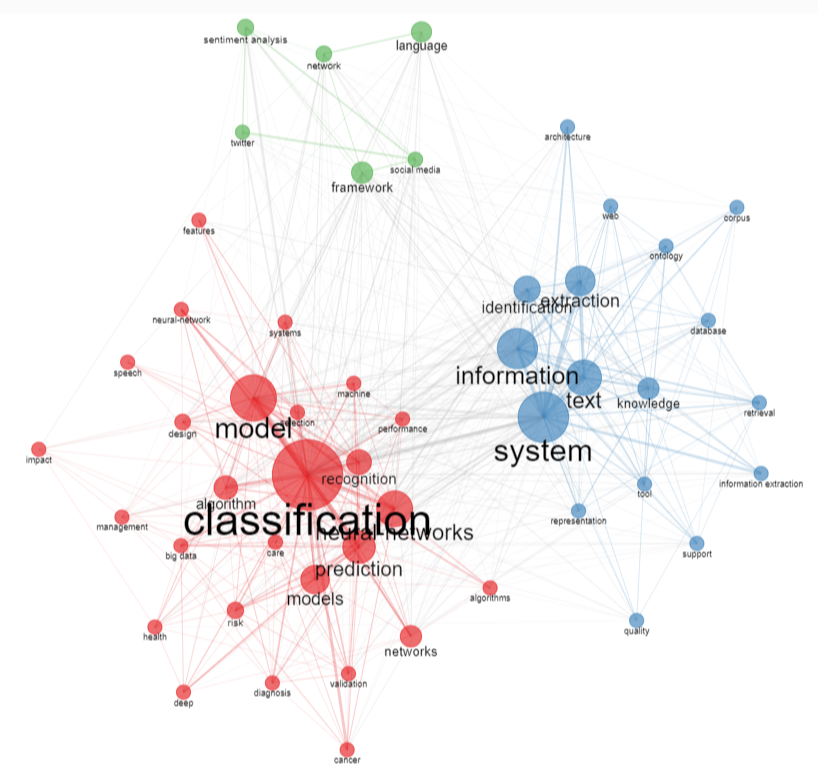
\includegraphics[width=1\textwidth]{experiments/ABMHub/PesquisaBibliometrica/NLP/grafo_keywords.png}
    \caption{Grafo de relação de keywords}
    \label{fig:ABMHub:NLPgraph1}
\end{figure}

Assim, é necessário uma nova iteração da pesquisa, para evitar que registros de visão computacional corrompam a pesquisa de NLP. É delicado fazer isso, pois existem muitas menções a Visão Computacional nos registros de LP, já que ambos são ligados a Deep Learning, então retirar a keyword "Visão Computacional" provavelmente removeria muitos registros que não gostaríamos de remover da pesquisa. Assim, a melhor solução encontrada foi remover palavras que não têm intersecção entre os dois assuntos. Por exemplo, "medical", "cancer" e "diagnosis".

Assim, chegamos na mais recente query:

\lstinputlisting[numbers=left,basicstyle=\normalsize\ttfamily,caption={Query refinada de busca sobre Procesasmento de Linguagem Natural.},label=queryRefinadaNLP03022022]
{experiments/ABMHub/PesquisaBibliometrica/NLP/pesquisa_nova.txt}

Esta query refinada retornou 8557 registros.

\subsection{Filtragem de registros}

Após a refinagem, foi estabelecido que usaremos o dataset de 8557 registros. Portanto, podemos começar a tratá-lo e analisá-lo. Para isso, começamos filtrando registros indesejados, como prévias de artigos, críticas sobre outros arquivos, cartas e etc. Assim, deixaremos apenas os artigos, pois é o método padrão de publicação científica, e capítulos de livros, já que é um tipo de publicação recorrente na área. Após o filtro, reduzimos nosso dataset para 3308 registros. A partir deste ponto, o "dataset" mencionado será o dataset filtrado.

\subsection{Análise descritiva do \textit{dataset}}

Ainda utilizando a ferramenta Bibliometrix, faremos uma análise descritiva do dataset adquirido, ou seja cálculos de diversas métricas para trazer \textit{insights}.

\begin{description}
    \item [\textit{Timespan}] De 1990 até 2022 (hoje). Não foram encontrados registros de 1945 até 1989.
    \item [\textit{Sources (Journals, Books, etc)}] 750 fontes diferentes de artigos.
    \item [\textit{Average years from publication}] A média do tempo de publicação dosartigos no dataset é de 3,85 anos.
    \item [\textit{Average citations per documents}] Cada artigo foi citado em média 14.03 vezes.
    \item [\textit{Average citations per year per doc}] Os artigos do dataset por inteiro são, em média, citados 2567 vezes por ano.
    \item [\textit{References}] Os artigos têm 108452 referência para outras fontes.
    \item [\textit{Keywords Plus (ID)}] Há 2414 diferentes palavras chaves.
    \item [\textit{Author's Keywords (DE)}] Há 7439 diferentes palavras chaves, segundo os autores.
    \item [\textit{Authors}] Há 10028 diferentes autores.
    \item [\textit{Author Appearances}] Há 13237 autores (considerando repetição nomes para diferentes artigos).
    \item [\textit{Authors of single-authored documents}] Há 154 autores que fizeram trabalhos sozinhos.
    \item [\textit{Authors of multi-authored documents}] Há 9874 autores que fizeram trabalhos com outras pessoas.
    \item [\textit{Single-authored documents}] Há 163 trabalhos com apenas um autor.
    \item [\textit{Documents per Author}] Há, em média, 0,33 autores por trabalho.
    \item [\textit{Authors per Document}] Há, em média, 3,03 trabalhos por autor.
    \item [\textit{Co-Authors per Documents}] As 13237 aparições de autores se distribuem, em média 4 vezes para os 3308 documentos do dataset.
    \item [\textit{Collaboration Index}] Os autores que editaram artigos com um ou mais co-autores, colaboraram em media 3,54 vezes para editar os elaborados em co-autoria.
\end{description}

\subsection{Evolução da Produção Científica}


A evolução da produção científica do assunto é um dos principais motivadores dessa pesquisa. Afinal, com a quantidade absurda de dados que existem hoje livremente disponíveis na internet (e em exponencial crescimento), provavelmente influencia muito a qualidade de modelos gerados em qualquer área de machine learning. É esperado que, motivado por essa crescente de dados, e com a popularização de assistentes virtuais, NLP seja um tópico cada vez mais estudado.

 \begin{figure}
    \centering
    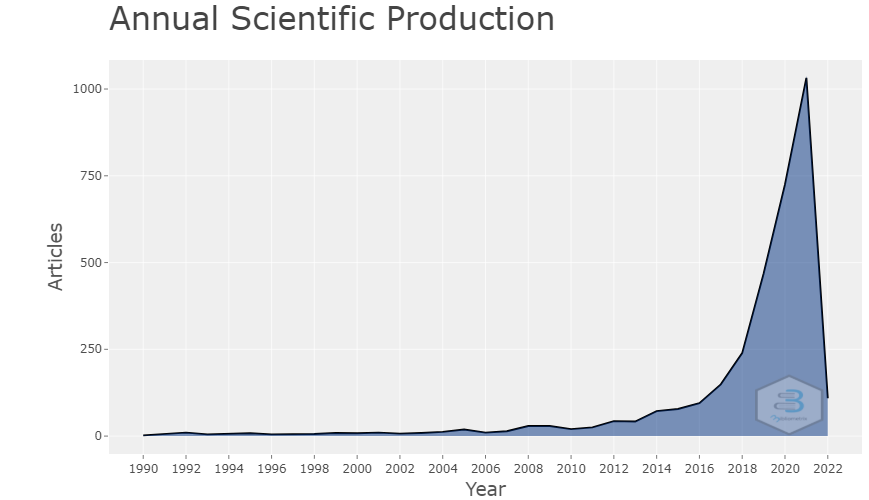
\includegraphics[width=1\textwidth]{experiments/ABMHub/PesquisaBibliometrica/NLP/anualScientificProduction.png}
    \caption{Produção científica anual}
    \label{fig:ABMHub:ASP}
\end{figure}

Podemos ver que as suposições anteriores são verdadeiras (ou, ao menos, aparentemente verdadeiras). Como visto na figura \ref{fig:ABMHub:ASP}, a crescente absurda e exponencial em deep learning entre 2016 e 2021 realmente dá pistas que NLP está cada vez mais relevante no mundo moderno, e que continuará crescendo em influência por um bom tempo. É importante ressaltar que a queda apresentada no fim do gráfico ocorre apenas porque esses registros foram extraídos no começo do ano 2022.

Também é interessante observar que o primeiro registro é em 1990. O conceito de NLP foi inventado antes dessa data, mas apenas a partir desse ponto que NLP começou a ser estudado junto com Machine Learning, e a query utilizada (seção \ref{sec:ABMHub:query}) especifica que é necessária a ligação de processamento de linguagem natural com inteligência artificial.

\subsection{Evolução das Citações}

 \begin{figure}
    \centering
    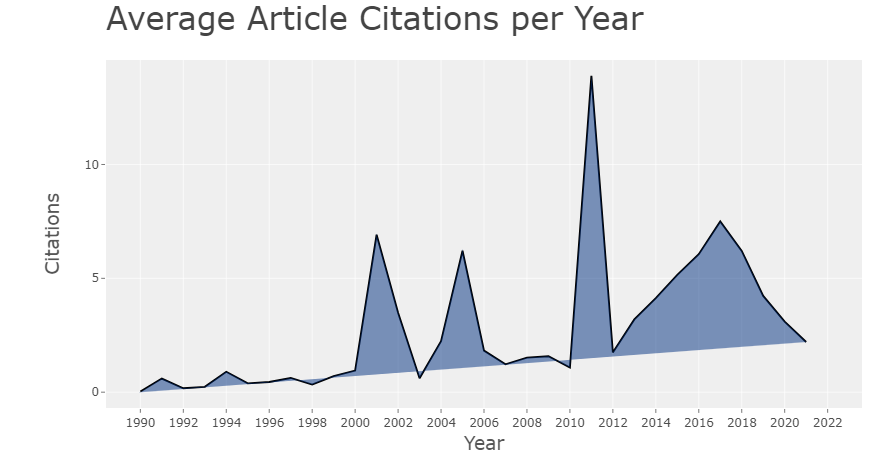
\includegraphics[width=1\textwidth]{experiments/ABMHub/PesquisaBibliometrica/NLP/citationsPerYear.png}
    \caption{Produção científica anual}
    \label{fig:ABMHub:CPY}
\end{figure}

Podemos perceber que há um claro crescimento médio desde 1990 das citações médias por ano. Uma das coisas que mais chama atenção são os 4 picos no gráfico: em 2001, 2005, 2011 e 2017. Esses provavelmente são de artigos (ou grupos de artigos) que tiveram um impacto fora do comum, trazendo novos conceitos ou realizando descobertas fantásticas.

Esta é, inclusive, uma das perguntas feitas como motivação de pesquisa: "Como se dá o progresso das pesquisas em NLP ao longo dos anos? As redes sociais influenciaram esse crescimento?". Vemos que há crescimento mas, exclusivamente através desses dados, é difícil tirar conclusões sobre a relação deste crescimento com a vinda de redes sociais. 

\subsection{\textit{Three-Field Plots (Sankey diagram)}}

Como o nome indica, "Three-Field Plots" são tipos de gráficos que buscam correlacionar três tipos de dados diferentes, sem a necessidade de uma terceira dimensão adicionada em cima de um gráfico bidimensional. Na imagem \ref{fig:ABMHub:TFP}, temos um exemplo de plotagem de três campos que interliga os autores presentes no dataset, com fontes que eles citaram, assim como palavras chaves que costumam usar em seus artigos. 

 \begin{figure}
    \centering
    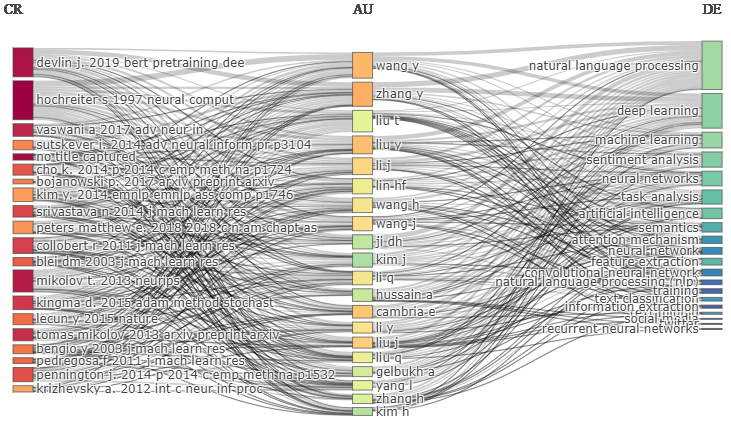
\includegraphics[width=1\textwidth]{experiments/ABMHub/PesquisaBibliometrica/NLP/tfp1.png}
    \caption{Three Field Plot - Citações, Autores e Palavras chaves}
    \label{fig:ABMHub:TFP1}
\end{figure}

Nessa plotagem, podemos extrair algumas informações muito interessantes sobre o estado atual de NLP. Primeiramente, vemos que o artigo mais citado por todos os artigos do dataset aqui apresentado é sobre computação neural (ou redes neurais), o que faz muito sentido, considerando que a NLP moderna é baseada em machine e deep learning. Outra observação interessante é que os artigos, em geral, são igualmente citados, mostrando que existe uma série de conceitos base para a NLP que são usados na maioria das aplicações do conceito.

Outro ponto interessante é que quase todos os autores listados no gráfico são chineses. Isso evidencia muito claramente a ascensão da China como potencia intelectual e tecnológica, principalmente em uma área tão relevante como a Inteligência Artificial.

Por último, as keywords também merecem sua atenção. Como esperado por ser o foco do dataset, Processamento de Linguagem Natural é a palavra-chave com mais menções. Mas, em seguida, vemos "Deep Learning", "Machine Learning" e "Neural Networks", o que faz muito sentido, partindo do princípio que (como dito anteriormente), NLP se apoia nesses conceitos atualmente. Também temos, com tamanho considerável, "sentiment analysis" e "task analysis", que são aplicações muito famosas de NLP.